\documentclass{amsart}

\textheight=22.5cm
\topmargin=0.5cm

\usepackage{amssymb}
\usepackage{graphicx,color}
\usepackage{amsmath}
\usepackage{url}
\usepackage[colorlinks=true]{hyperref}

\usepackage{cleveref}
\Crefname{counterexample}{counterexample}{counterexamples}
\Crefname{counterexample}{Counterexample}{Counterexamples}
\Crefname{conjecture}{conjecture}{conjectures}
\Crefname{conjecture}{Conjecture}{Conjectures}


\usepackage{tikz-cd}
\usepackage{tikz}
\usetikzlibrary{matrix}
\usepackage{tkz-euclide}



\newcommand{\limites}{}

\theoremstyle{plain}
\newtheorem{theorem}{Theorem}[section]
\newtheorem{proposition}[theorem]{Proposition}
\newtheorem{lemma}[theorem]{Lemma}
\newtheorem{corollary}[theorem]{Corollary}
\newtheorem{claim}[theorem]{Claim}

\theoremstyle{definition}
\newtheorem{definition}[theorem]{Definition}
\newtheorem{notation}[theorem]{Notation}
\newtheorem{example}[theorem]{Example}
\newtheorem{problem}[theorem]{Problem}
\newtheorem{question}[theorem]{Question}
\newtheorem{conjecture}[theorem]{Conjecture}
\newtheorem{remark}[theorem]{Remark}


% Macros in general

\newcommand{\F}{ \ensuremath{\mathbb{F}}}
\newcommand{\N}{ \ensuremath{\mathbb{N}}}
\newcommand{\Z}{ \ensuremath{\mathbb{Z}}}
\newcommand{\C}{ \ensuremath{\mathbb{C}}}
\newcommand{\R}{ \ensuremath{\mathbb{R}}}

\newcommand{\T}{ \ensuremath{\mathcal{T}}}

\newcommand{\bb}{{\mathbf{b}}}
\newcommand{\cc}{{\mathbf{c}}}
\newcommand{\ttt}{\mathbf{t}}
\newcommand{\GL}{{GL}_r (K)}

\renewcommand{\int}{\operatorname{int}}
\newcommand{\width}{\operatorname{width}}
\newcommand{\ind}{\operatorname{index}}
\newcommand{\Vol}{\operatorname{Vol}}
\newcommand{\length}{\operatorname{length}}


\newcommand{\cone}{\ensuremath{\mathrm{cone}}\hspace{1pt}}
\newcommand{\conv}{\ensuremath{\mathrm{conv}}\hspace{1pt}}
\newcommand{\cayley}{\operatorname{Cay}}
\newcommand{\rank}{\operatorname{rank}}
\newcommand{\reg}{\operatorname{reg}}

\newcommand{\Image}{\ensuremath{\mathrm{Im}}\hspace{1pt}}

\usepackage[colorinlistoftodos]{todonotes}

\newcommand{\giulia}[1]{\todo[size=\tiny,color=blue!30]{#1 \\ \hfill --- G.}}
\newcommand{\Giulia}[1]{\todo[size=\tiny,inline,color=blue!30]{#1 \\ \hfill --- G.}}

\newcommand{\paco}[1]{\todo[size=\tiny,color=green!30]{#1 \\ \hfill --- P.}}
\newcommand{\Paco}[1]{\todo[size=\tiny,inline,color=green!30]{#1 \\ \hfill --- P.}}



\date{\today}

\author[G.~Codenotti]{Giulia Codenotti}
\author[F.~Santos]{Francisco Santos}

\address[G.~Codenotti]
{
Institut f\"ur Mathematik, Freie Universit\"at Berlin, Germany
}
\email{giulia.codenotti@fu-berlin.de}

\address[F.~Santos]
{
Department of Mathematics, Statistics and Computer Science, University of Cantabria, Spain
}
\email{francisco.santos@unican.es}

\thanks{The authors were supported by the Einstein Foundation Berlin under grant EVF-2015-230. 
Work of F. Santos is also supported by project MTM2017-83750-P of the Spanish Ministry of Science (AEI/FEDER, UE)}

%%%%%%%%%%%%%%%%%%%%%%%%%%%%%%%%%%%%%%%%%%%%%%%%%%%%%%%%%%%

\title{Unimodular covers of 3-dimensional parallelepipeds and Cayley sums}

\begin{document}

\begin{abstract}
We show that the following classes of three-dimensional lattice polytopes have unimodular covers: the class of all parallelepipeds, the class of all centrally symmetric polytopes, and the class of all three-dimensional Cayley sums $\cayley(P,Q)$ where the normal fan of $Q$ refines that of $P$. This improves results of Beck et al. (2018) and Haase et al. (2008) where the last two classes were shown to be IDP.
\end{abstract}

\maketitle

\section{Introduction}

A lattice polytope $P\subset \R^d$ has the \emph{integer decomposition property} if for every positive integer $n$, every lattice point $p \in nP\cap \Z^d$ can be written as a sum of $n$ lattice points in $P$. We abbreviate this by saying that ``$P$ is IDP''. Being IDP is interesting in the context of  both enumerative combinatorics (Ehrhart theory) and algebraic geometry (normality of toric varieties) and it falls into a hierarchy of several properties each stronger than the previous one. See, e.g., \cite[Sect. 1.2.5]{HPPS-survey}, \cite[p. 2097]{mfo2004}, \cite[p. 2313]{mfo2007}.
\paco{cite Bruns-Gubeladze book?}
Let us here only mention that
\[
P \text{ has a unimodular triangulation}\Rightarrow
P \text{ has a unimodular cover}\Rightarrow
P \text{ is IDP.}
\]
Remember that a \emph{unimodular triangulation} is a triangulation of $P$ into unimodular simplices, and a \emph{unimodular cover} is a collection of unimodular simplices whose union equals $P$. 

\paco{define mixed IDP, Cayley sums, Minkowski sums, mixed subdivisions}
A lattice polytope is called \emph{smooth} if it is simple and the edge generators at every vertex form a linear basis for the lattice. 
%
Oda~\cite{Oda1997} posed several questions regarding IDP polytopes which are now considered conjectures (REFERENCES). 
Among them:
\begin{conjecture}
\label{conj:Oda}
\begin{enumerate}
\item (Related to problems 1, 3, 4, 6 in \cite{Oda1997}) Let $P, Q\subset \R^d$ be lattice polytopes with the normal fan of $Q$ refining that of $P$, and $P$ smooth. Then
\begin{align*}
\label{eq:mixedIDP}
(P+Q) \cap \Z^d = P \cap \Z^d + Q \cap \Z^d.
\end{align*}
\paco{perhaps we can call this formula ``being mixed IDP''. The property of ``$N(Q)$ refines $N(P)$'' is sometimes called ``$P$ is a Minkowski summand of $Q$''.}

\item (Related to problems 2 and 5 in \cite{Oda1997})
Every smooth lattice polytope is IDP.
\end{enumerate}
\end{conjecture}

Motivated by these and other questions, several authors have studied the IDP property for different classes of lattice polytopes. 

For example,  very recently
Beck et al.~\cite{BHHHJKM2019} proved that all smooth centrally symmetric $3$-polytopes are IDP.
More precisely, they show that any such polytope can be covered by lattice 
parallelepipeds and unimodular simplices, both of which are trivially IDP.

Partially motivated by this result in \Cref{sec:parallelepipeds} we show:

\begin{theorem}
\label{thm:parallelepipeds}
Every $3$-dimensional lattice parallelepiped has a unimodular cover.
\end{theorem}

As a consequence:

\begin{corollary}
\label{coro:3cs}
Every smooth centrally symmetric lattice $3$-polytope has a unimodular cover. 
\qed
\end{corollary}

\begin{question}
Do $3$-dimensional parallelepipeds have unimodular triangulations?
\end{question}

\begin{question}
Higher dimensional parallelotopes (affine images of cubes) are IDP. Do they have unimodular covers? 
\end{question}

%\begin{proof}
%Let $P$ be a smooth centrally symmetric lattice $3$-polytope.
%Beck et al.~\cite{BHHHJKM2019} show that $P$ is IDP by covering it with parallelepipeds and unimodular simplices. Once we know parallelepipeds have unimodular covers (\Cref{thm:parallelepipeds}), we conclude $P$ has a unimodular cover too.
%\end{proof}

Another case of Oda's questions that has been solved is the two-dimensional case of \Cref{conj:Oda}(1), with three different proofs by
Fakhruddin~\cite{Fakhruddin}, Ogata~\cite{Ogata} and Haase et al.~\cite{HNPS2008}, the latter without assuming $P$ smooth. 
In dimension three however the statement fails without the smoothness assumptin, as shown by letting $P=Q$ be the empty simplex of volume two.

An alternative approach to \Cref{conj:Oda}(1) is via Cayley sums. As we note in \Cref{sec:cayley} (\Cref{prop:mixedIDP}), if $P,Q\subset \R^d$ are two lattice polytopes one has
\[
\cayley(P,Q) \text{ is IDP} 
\Rightarrow
(P+Q) \cap \Z^d = P \cap \Z^d + Q \cap \Z^d.
\]
In \Cref{sec:cayley} we show the following even stronger result, in the two-dimensional case:

\begin{theorem}
\label{thm:cayley}
Let $P$ and $Q$ be lattice polygons with the normal fan of $Q$ refining that of $P$. Then the Cayley sum $\cayley(P,Q)$ has a unimodular cover.
\end{theorem}

As an application of this, we prove \Cref{conj:Oda}(2) for $3$-dimensional \emph{prismatoids}, polytopes whose vertices all lie in two parallel facets:

\begin{corollary}
\label{coro:prismatoid}
Every smooth $3$-dimensional lattice prismatoid has a unimodular cover.
\end{corollary}

\Paco{another corollary, suggested by Christian Haase: the $k$-th dilation of an emptyy simplex is very easy to decompose into slices of width one all of which fit into our description ($P$ and $Q$ are either pararllel parallelograms, one of which perhaps degenerates to a segment). In particular, we recover as a corollary that the $k$-th dilation of every empty tetrahedron (and, a fortiori, the $k$-th dilation of every lattice $3$-polytope) has a unimodular cover for every $k\ge 2$}


We believe that the $3$-polytopes in these four statements all have unimodular triangulations, but we do not have a proof.


\subsection*{Acknowledgements:} We thank Akiyoshi Tsuchiya, Spencer Backman, Gaku Liu, Johannes Hofscheier, Christian Haase, .... et al.

%\section{Preliminaries}
%\label{sec:prelim}


\section{Parallelepipeds}
\label{sec:parallelepipeds}

The main tool is what we call the parallelepiped circumscribed to a given tetrahedron, defined as follows:

\begin{definition}
Let $T$ be a tetrahedron with vertex set $p_1,p_2,p_3,p_4$. Consider points $q_1,q_2,q_3,q_4$ defined as $q_i= \frac12 (p_1+p_2+p_3+p_4) - p_i$ and define 

\[
C(T)=\conv(p_i,q_i: i\in[4]).
\] 

$C(T)$ is a parallelepiped whose faces are of the form $\conv(p_i, p_j, q_k, q_l)$ for all $\{i,j,k,l\}=[4]$, which we call the \emph{parallelepiped circumscribed} to $T$.

For each $i \in [4]$, let $T_i=\conv(q_i, p_j, p_k, p_l)$, with $\{i,j,k,l\}=[4]$; we call these $T_i$ the \emph{corner tetrahedra} of $C(T)$. These along with $T$ form a triangulation of $C(T)$.
\end{definition}
\paco{define the ``corner tetrahedra''}

The idea to have in mind is that of the regular tetrahedron inscribed in a cube. Modulo an affine transformation this is exactly the situation of $T$ and $S$.
\giulia{we should add a picture of the standard cube}

\Giulia{not sure if we need this remark:
$S$ is ``half a fundamental domain'' for the affine lattice $\Lambda_P$ generated by $p_1,\dots,p_4$, in the following precise sense: if $x$ is an arbitrary point, then $S$ intersects either $\Lambda_P + x$ or $\Lambda_P -x$ (and, if $x$ is generic then the intersection is unique). Proof: think of this property for the standard cube and the lattice $\{sum of coordinates is even\}$ generated by the vertices of the regular tetrahedron inscribed in it. (Remark: let us assume without loss of generality that $\Lambda_P$ contains the origin, so that $\Lambda + x$ is the class of $x$ modulo $\Lambda$).
}

\begin{lemma}
\label{lemma:corner}
Let $T=\conv\{p_1,p_2,p_3,p_4\}$ be an empty lattice tetrahedron that is not unimodular and $C(T)$ be the parallelepiped circumscribed to $T$. Let $T_1, T_2,T_3$ and $T_4$ be the corresponding corner tetrahedra in $C(T)$. Then, every $T_i$ contains at least one lattice point different from $\{p_1,\dots,p_4\}$.
\end{lemma}

\begin{proof}
By White's classification of empty tetrahedra (\cite{White1964}, see also, e.~g.~\cite[Sect.~4.1]{HPPS-survey}), there is no loss of generality in assuming $T=\conv(p_1,p_2,p_3,p_4)$ with
\[
p_1=(0,0,0), \quad
p_2=(1,0,0), \quad
p_3=(0,0,1), \quad
p_4=(a,b,1).
\]
where $b\ge 2$ is the (normalized) volume of $T$, and $a\in \{1,\dots,b-1\}$ satisfies $\gcd(a,b)=1$. This gives 
\paco{picture of the quadrilaterals $p_1q_4p_2q_3$ and $q_2p_3q_1p_4$ would be good.}
\begin{align*}
q_1=\left(\frac{1+a}2,\frac{b}2,1\right), &&
q_2=\left(\frac{a-1}2,\frac{b}2,1\right), \quad\\
q_3=\left(\frac{1+a}2,\frac{b}2,0\right), &&
q_4=\left(\frac{1-a}2,-\frac{b}2,0\right).
\end{align*}

Then, the inequalities $b\ge 1+a$ and $b\ge 2$ imply:
\[
(1,1,0)\in \conv(p_1p_2q_3) \subset T_4, \quad
(0,-1,0)\in \conv(p_1p_2q_4) \subset T_3.
\]
\paco{Alternative arguments: one can explicitly compute coordinates of lattice points in $T_1$ and $T_2$, or one can say that the isomorphism $T_{a,b} \cong T_{a^{-1},b}$ of White tetrahedra exchanges the edges at $\{z=0\}$ and at $\{z=1\}$.}
Now, this implies that the quadrilateral $\conv(p_1q_4p_2q_3)$ contains a fundamental domain for the lattice $\Z^2\times\{0\}$. Hence, its translate $\conv(q_2p_3q_1p_4)$ contains a fundamental domain for $\Z^2\times\{1\}$ and, in particular, it contains at least one lattice point other than $p_3$ and $p_4$. By central symmetry around its center $\left(\frac{a}2,-\frac{b}2,1\right)$, $\conv(q_2p_3q_1p_4)$ must contain lattice points in both triangles $\conv(q_2p_3p_4)\subset T_1$ and $\conv(q_1p_3p_4)\subset T_2$.
\end{proof}


\begin{lemma}
\label{lemma:3<4}
Let $P$ be a lattice parallelepiped and let $T\subset P$ be an empty tetrahedron. Then, at least one of the four corner tetrahedra $T_i$ of the circumscribed parallelogram $C(T)$ is fully contained in $P$.
\end{lemma}

\begin{proof}
We denote the vertices of $T$ by $p_1, p_2, p_3, p_4$ and by $q_1, q_2, q_3, q_4$ the vertices of $C(T)$ not in $T$, as before. Let $f\in (\R^3)^*$ be any functional. Fix $i \in [4]$; observe that if $f(q_i) > f( p_j)$ for all $j\neq i$, then 
\begin{gather*}
f(q_i) \overset{(i)}{>} f(q_j) \overset{(ii)}{>} f(p_i) \\
f(q_i) \overset{(iii)}{>} f(p_j) \overset{(iv)}{>} f(p_i) \\
f(p_j)\overset{(v)}{>}f(q_k)
\end{gather*}
for all $j \neq i$, $k \notin \{j, i\}$. 

Indeed, for any $\{i,j,k,l\}=[4]$ we have 

\begin{align*}
f(q_i) > f( p_j) \Leftrightarrow \frac12 f(p_l+&p_k -p_j-p_i) > 0  \Leftrightarrow f(q_j) > f(p_i)\\
& \Updownarrow \\
 f(q_l) < f(p_k) \Leftrightarrow \frac12 f(-p_l-&p_k +p_j+p_i) < 0 \Leftrightarrow f(q_k) < f(p_l),
\end{align*}
which shows the equivalence of $(i)$, $(iii)$ and $(v)$; note that $(iii)$ is our assumption. Inequalities $(ii)$ and $(iv)$ follow by taking the sum of two inequalities of the form $\frac12 f(p_l+p_k -p_j-p_i) > 0$. 

Using this observation, we can show that each of pairs of parallel facets of $P$ cuts out at most one of the $q_i$s:
if $q_i$ lies outside of $P$, it must violate a facet-defining inequality $f(x) \leq a$.Thus $f(q_i) > a \geq f(p_j)$, and by our observation, it follows that all remaining $q_j$ satisfy the inequality $f(x) \leq a$. Since $P$ is a parallelogram, there is a facet with inequality $f(x) \geq b$; by what is said above, the minimum value of $f(x)$ is attained at $p_i$, which is in $P$. Thus $f(q_j) > f(p_i) \geq b$, that is, the inequality is satisfied by all the $q_j$.

Since at most one of the $q_i$ does not satisfy the inequalities corresponding to a pairs of parallel facets of $P$, and there are only three pairs of facets, one of $q_i$s must satisfy all the inequalities and therefore be inside of $P$.
\end{proof}
\giulia{here it may also be nice to add a picture}

\begin{proof}[Proof of \Cref{thm:parallelepipeds}]
Let $P \subseteq \R^3$ be a parallelopiped. It can be triangulated into empty lattice tetrahedra, simply by taking a triangulation which uses all lattice points as vertices.  If all the tetrahedra in the triangulation are unimodular we are done. Otherwise, suppose $T$ is be empty tetrahedron in the triangulation which is not unimodular. \Cref{lemma:3<4} guarantees that one of the corner tetrahedra $T_i$ of the parallelepiped $C(T)$ circumscribed to $T$ is contained in $P$. Without loss of generality, suppose $T_4 = \conv(p_1, p_2, p_3,q_4)$ is in $P$. By \Cref{lemma:corner}, we know that $T_4$ contains a lattice point, which we denote by $l$. Observe that from the proof of \Cref{lemma:corner} we know more: $l$ lies in the face $\conv(p_1, p_2, q_4)$.\giulia{we need this for the volume computation below. perhaps it should be made explicit in the statemente of the lemma...}

Then $S=\conv(T\cup \{l\})$ can be triangulated in two different ways: $S=T \cup T'_4 = S_1 \cup S_2 \cup S_3$, where $T'_4 = \conv(p_1, p_2, p_3, l) \subseteq T_4$ and
\[
S_1= \conv(p_2,p_3,p_4, l),
S_2=\conv(p_1,p_3,p_4, l),
S_3=\conv(p_1,p_2,p_4, l).
\]

Each of the tetrahedra $S_i$ has lattice volume strictly smaller than $T$: indeed, $\Vol(S_3)=\Vol(T'_4)$, since these tetrahedra have a common face $\conv(p_1, p_2, l)$ and the remaining vertex is at distance one from this face in both. Now $T'_4$ is contained in $T_4$, and we know that each corner tetrahedron $T_i$ has volume half that of $T$. The remaining two tetrahedra $S_1$ and $S_2$ must therefore have volume summing to that of $T$, and therefore each has volume strictly less than $T$.

This allows us to cover $T$ with lattice simplices of smaller volume recursively, until it is covered by unimodular ones.
\end{proof}

\begin{remark}
\label{rem:octahedra_and_tri-prisms}
Let us say that a lattice $3$-polytope $P$ \emph{has the circumscribed parallelepiped property} if it satisfies the conclusion of \Cref{lemma:3<4}:  ``for every empty tetrahedron $T$ contained in $P$ at least one of the four corner tetrahedra in $C(T)$ is 
contained in $P$''. Then $P$ has a unimodular cover, since the proof of \Cref{thm:parallelepipeds} works for $P$.

In turn, our proof of \Cref{lemma:3<4} relies on the fact that parallelepipeds have only three (pairs of) normal vectors. The proof fails if $P$ has four of them, as the following non-IDP octahedron and triangular prism show:

\begin{example}
\label{ex:non-IDP}
The following lattice octahedron is not IDP:
\[
Q= \conv((0,1,1),(1,0,1),(1,1,0),(0,-1,-1),(-1,0,-1),(-1,-1,0))
\]

The following lattice triangular prism is not IDP:
\[
P=\conv((0,1,1),(1,0,1),(1,1,0),(-1,0,0),(0,-1,0),(0,0,-1)).
\]
Indeed, in both polytopes the only lattice points are the six vertices and the origin. The point $(1,1,1)$ lies in the second dilation but is not the sum of two lattice points in the polytope.
\giulia{is it necessary to be more explicit, for example show that these are the only lattice points?}
\end{example}

\end{remark}

\begin{question}
Does every smooth 3-polytope have the circumscribed parallelepiped property? By the above remark, if the answer is yes then every smooth $3$-polytope has a unimodular cover.
\end{question}


\section{nef Cayley sums}
\label{sec:cayley}

Throughout this section let $P$ and $Q$ be two lattice polytopes in $\R^d$. We do not require them to be full-dimensional, but we assume their Minkowski sum is. Remember that the Minkowski sum $P+Q$ of $P$ and $Q$ is defined as:
\[
P + Q := \{ p+q \in \R^d: p\in P, q \in Q\}.
\]
The \emph{Cayley sum} of $P$ and $Q$ is defined as
\[
\cayley (P,Q) = \conv( P\times\{0\} \cup Q\times \{1\}) \in \R^{d+1}.
\]
The assumption that $P+Q$ is $d$-dimensional is equivalent to $\cayley (P,Q)$ is a $(d+1)$-dimensional.

We introduce the following two concepts.

\begin{definition}
In the above conditions, we say that $Q$ \emph{is nef for $P$} if the normal fan of $Q$ refines that of $P$. If this happens, we say that $\cayley(P,Q)$ is a \emph{nef Cayley sum}.

We say that the pair $(P,Q)$ is \emph{mixed IDP} if 
\paco{``mixed IDP'' is not the right property, since this is weaker than IDP}
\[
(P\cap \Z^d) + (Q\cap \Z^d) = (P+Q)\cap \Z^d.
\]
\end{definition}

In this language, \Cref{conj:Oda}(1) translates to:
\emph{If $Q$ is nef for $P$ and $P$ is smooth then the pair $(P,Q)$ mixed IDP.}


\begin{proposition}
\label{prop:mixedIDP}
If $\cayley(P,Q)$ is IDP then the pair $(P,Q)$ is mixed IDP.
\end{proposition}

The so-called \emph{Cayley Trick} is the isomorphism
\[
2\cayley(P, Q) \cap (\R^d\times \{1\}) \cong P+Q,
\]
which induces the following canonical bijections:
\begin{align*}
\text{polyhedral subdivisions of $\cayley(P,Q)$} &\leftrightarrow \text{mixed subdivisions of $P + Q$}\\
\text{triangulations of $\cayley(P,Q)$} &\leftrightarrow \text{fine mixed subdivisions of $P + Q$}\\
\text{unimodular simplices in $\cayley(P,Q)$} &\leftrightarrow \text{unimodular prod-simplices in $P + Q$}.
\end{align*}
See \cite{DLRS2010} for more details on the Cayley Trick and on triangulations and polyhedral subdivisions of polytopes.
In fact these bijections can be taken as definitions of the objects in the right-hand sides. In particular, 
we call \emph{prod-simplices} in $P+Q$ the Minkowski sums $T_1+T_2$ where $T_1\subset P$ and $T_2\subset Q$ are simplices with complementary affine spans. A prod-simplex is \emph{unimodular} if the edge vectors from a vertex of $T_1$ and from a vertex of $T_2$ form a unimodular basis.

%As a consequence, we also have that:
%\begin{align*}
%\text{$\cayley(P,Q)$ has a unimodular cover} &\leftrightarrow \text{$P+Q$ can be covered by unimodular prod-simplices}.
%\end{align*}

Our proof of \Cref{thm:cayley} is based on the following result:

\begin{figure}[htb]
  \centering
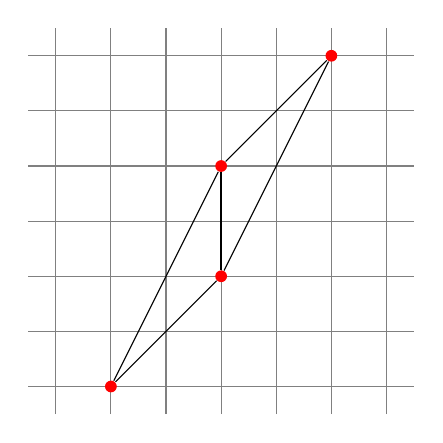
\begin{tikzpicture}[mynode/.style={circle, inner sep=1.5pt, fill=red}, scale =
  .7]
%coordinate axes
   \tkzInit[xmax=3.5,ymax=3.5,xmin=-3.5,ymin=-3.5]
%        \tkzLabelX[orig=false,label options={font=\tiny}]
%        \tkzLabelY[orig=false,label options={font=\tiny}]
        \tkzGrid
%       \tkzDrawX
%       \tkzDrawY

%hexagon
  \node[mynode] (A) at (0,-1) {}; 
%  \node[mynode] (B) at (1,1) {};  
  \node[mynode] (C) at (2,3) {};  
  \node[mynode] (D) at (0,1) {};  
%  \node[mynode] (E) at (-1,-1) {};  
  \node[mynode] (F) at (-2,-3) {};  

%other points
%  \node[mynode] () at (0,-1) {}; 


  \draw[black] (A) -- (C) -- (D) -- (F) -- (A);
  \draw[black, thick] (A) -- (D);
\end{tikzpicture}
%
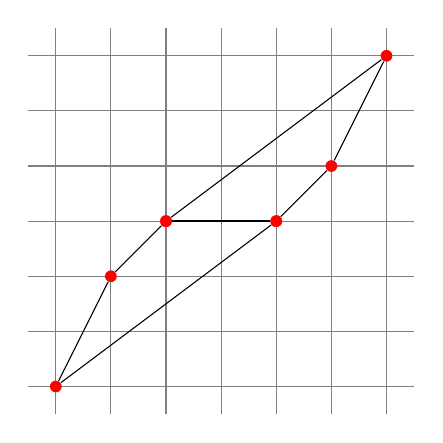
\begin{tikzpicture}[mynode/.style={circle, inner sep=1.5pt, fill=red}, scale =
  .7]
%coordinate axes
   \tkzInit[xmax=3.5,ymax=3.5,xmin=-3.5,ymin=-3.5]
%        \tkzLabelX[orig=false,label options={font=\tiny}]
%        \tkzLabelY[orig=false,label options={font=\tiny}]
        \tkzGrid
%        \tkzDrawX
%        \tkzDrawY

%hexagon
  \node[mynode] (A) at (1,0) {}; 
  \node[mynode] (B) at (2,1) {};  
  \node[mynode] (C) at (3,3) {};  
  \node[mynode] (D) at (-1,0) {};  
  \node[mynode] (E) at (-2,-1) {};  
  \node[mynode] (F) at (-3,-3) {};  

  \node[mynode] (p1) at (-1,0) {}; 
  \node[mynode] (p2) at (1,0) {};  

  \draw[black] (A) -- (B) -- (C) -- (D) -- (E) -- (F) -- (A);
  \draw[black, thick] (p1) -- (p2);
\end{tikzpicture}

\centerline{\hfill $P$ \hfill\hfill $Q$ \hfill}

\caption{Partial counter-example to \Cref{lemma:cayley}. With respect to the standard lattice it is not a counter-example because (a) the edges $p_1p_2$ and $q_1q_2$ are not primitive and (b) the origin is a lattice point in the interior of both bands (but it is the only one). 
%
With respect to the lattice of index two it is not a counter-example either, because two vertices of $Q$ are not in that lattice.
}
\label{fig:width3}
\end{figure}

\begin{lemma}
\label{lemma:cayley}
Let $P$ and $Q$ be two lattice polygons with $Q$ nef with respect to $P$. Let $p_1p_2 \subset P$ and $q_1q_2\subset Q$ be two primitive and non-parallel segments, and assume that the prod-simplex (parallelogram)  $p_1p_2 + q_1q_2$ is not unimodular. Then,
at least one of the strips
\paco{add picture for these strips, and perhaps for the proof}
\[
(p_1p_2 + \langle \overrightarrow{q_1q_2}\rangle) \cap P
\qquad \text{or} \qquad
(q_1q_2 + \langle \overrightarrow{p_1p_2}\rangle) \cap Q
\]
has a lattice point in its interior.
\end{lemma}
\giulia{what I want is: a lattice point $p \in P$ such that either $p+q_1$ or $p+q_2$ lies in the interior of $\{p_1, p_2\} + \{q_1, q_2\}$ (or symmetric for $Q$)}

\begin{proof}
%Suppose by contradiction that there is no lattice point as described in the lemma. Then there cannot be a vertex of $P$ in the corresponding strip, since $P$ is a lattice polygon. The same holds for $Q$ and its corresponding strip. Thus $P$ has two edges which each have one vertex on each side of the strip $(p_1p_2 + \langle \overrightarrow{q_1q_2}\rangle)$; we will call these edges $e_1$ and $e_2$. The same holds for $Q$ and the strip $(q_1q_2 + \langle \overrightarrow{p_1p_2}\rangle)$, and we call the edges be $f_1, f_2$. 

Let us fix coordinates in which $p_1p_2$ and $q_1q_2$ are a vertical and horizontal segment of length one intersecting at the origin. That is, there are numbers $\alpha, \beta \in (0,1)$ such that
\[
p_1=(0,-\alpha), \quad
p_2=(0,1-\alpha), \quad
q_1=(-\beta,0), \quad
q_2=(1-\beta,0).
\] 
The ambient lattice is a certain lattice containing $p_1,p_2,q_1,q_2$ (the case of index two is when $\alpha=\beta=1/2$ and the lattice is spanned by these four points).

Suppose by contradiction that there is no lattice point as described in the lemma. Then there cannot be a vertex of $P$ in the corresponding strip, since $P$ is a lattice polygon. The same holds for $Q$ and its corresponding strip. Thus $P$ has two primitive edges which each have one vertex on each side of the strip $p_1p_2 + \langle \overrightarrow{q_1q_2}\rangle$; we will call these edges $\ell$ and $r$ (with $\ell$ to the left and $r$ to the right). The same holds for $Q$ and the strip $q_1q_2 + \langle \overrightarrow{p_1p_2}\rangle$, and we call the edges  $b, t$ (with $b$ below and $t$ above). To make things more explicit, we assume the following coordinates for the edge-vectors:
\[
\vec l = (l_1,l_2), \quad
\vec r= (r_1,r_2), \quad
\vec b= (b_1,b_2), \quad
\vec t= (t_1,t_2).
\]
Without loss of generality we assume $l_2,r_2,b_1,t_1 >0$. (They are non-zero and we can arbitrarily choose a sign for each vector).






Since the normal fan of $Q$ refines that of $P$, $Q$ will contain edges $e_1'$ and $e_2'$ parallel to $e_1$ and $e_2$ respectively. These edges of $Q$ are all distinct and appear alternating in $Q$, that is, they appear in the order $f_1, e_1', f_2, e_2'$. Indeed, consider the quadrilateral $S$ with vertices $q_1, p_1+l, q_2, p_2+l$, where $l$ is a lattice point chosen so that the segments $q_1q_2$ and $p_1+l,p_2+l$ intersect in their interior; we can further require that $\conv( q_1, p_1+l, q_2)$ is unimodular \giulia{not sure if we use it}. $S$ lies inside the $Q$-strip, while its translate $S-l$ lies inside the $P$-strip. Thus in order to have no lattice points in the strips, we must have that the edge $f_i$ separates the vertex $p_i +l$ of $S$ from the remaining three, and  the same for the edge $e_i +l$ and vertex $q_i$ of $S$. This is equivalent to saying that the normals to the edges $f_1, e_1, f_2, e_2$ lie in different open cones of the normal fan of $S$, in this cyclic order. 

- both $f_1$ or $f_2$ must meet the line through $q_1$ and $q_2$, else they would not cut out the lattice point they need to. same goes for $e_1$ and $e_2$ and the line through $p_1$ and $p_2$.

claim: the segments $e_1 + l$ and $e_2 + l$ respectively intersect both $f_1$ and $f_2$. 

claim: if we tilt one of the $f_i$s so that they are parallel, there is no room to fit $e_i$, since it intersects both. 





%Consider the segments on the lattice lines parallel to $p_1 p_2$ cut out by the edges $f_1$ and $f_2$ \giulia{this should be formulated more comprehensibly}. Since these segments do not contain lattice points, they must have lattice length stricly less than $1$ (or the width wrt $q$ is less than $k$, the index of $p,q$), which means that the smallest width in direction of $p_1 p_2$ between a "consecutive" vertices of $f_1$ and of $f_2$ must also be strictly less than $k$. 

%Further, we observe that both vertices of $f_1$ (or $f_2$) cannot lie strictly above the line through $q_1$ and $q_2$, else the strip would contain a lattice point. 
\end{proof}

\begin{proof}[Proof of \Cref{thm:cayley}]
Consider any lattice triangulation $\T$ of $\cayley(P,Q)$, or equivalently a mixed subdivision of $P+Q$. Observe that any simplex in $T$ has vertices in $Px\{0\}$ or in $Q \times \{1\}$, since $\cayley(P,Q)$ lies between two consecutive lattice hyperplanes $\{x_3=0\}$ and $\{x_3=1\}$. Thus simplices in $\T$ are of three types; they can , or have three vertices in $P$ and one in $Q$ (type $(3,1)$), have one vertex in $P$ and three in $Q$ (type $(1,3)$) or have two vertices in $P$ and two in $Q$ (type $(2,2)$). \giulia{is it usually denoted by dimension or cardinality? that is, (2,0) or (3,1)?} A triangulation of a simplex of type $(3,1)$ (resp $(1,3)$) is obtained by simply unimodularly triangulating the triangular face lying in $P$ (resp $Q$) and coning over the vertex in $Q$ (resp $P$). This leaves simplices of type $(2,2)$. In the mixed subdivision of $P+Q$ corresponding to $T$, these are mixed cells, that is parallelograms with one edge in $P$ and one in $Q$ \giulia{how imprecise can I be without being confusing?}.

Let $S=\{p_1, p_2\} + \{q_1, q_2\}$ be such a parallelogram. By \Cref{lemma:cayley} we know that there is a lattice point $p \in P$ such that either $p+q_1$ or $p+q_2$ lies in $S$, w.l.o.g. suppose it is $p+q_1$. Then we can cover $S$ by the triangle $\{p_1, p_2, p\} + q_1$ and parallelograms $\{p_1, p\}  + \{q_1, q_2\}$ and $\{p_2, p\} + \{q_1, q_2\}$. As above, the triangle can be unimodularly triangulated, while the volume of the two parallelograms sums up to the volume of $S$, and therefore each has volume strictly smaller than $S$. By iterating this procedure, we can cover $S$ by unimodular cells.
\end{proof}

\Cref{coro:prismatoid} is a particular case of the following situation. 
Let $Q_1$ and $Q_2$ be two polygons and consider the prismatoid 
\[
P= \conv(Q_1\times\{0\} \cup Q_2 \times \{k\},
\]
with $k\ge 2$. 
%Assume that $P\cap(\R^2\times\{i\})$ is a lattice polytope for every $i=0,\dots, k$. This is equivalent to assuming that $P\cap(\R^2\times\{1\})$ is a lattice polytope:

\begin{corollary}
If $P\cap(\R^2\times\{1\})$ is a lattice polygon then $P$ has a unimodular cover.
\end{corollary}

\begin{proof}
\paco{perhaps add details}
The condition that $P\cap(\R^2\times\{1\})$ is a lattice polygon implies the same for $P\cap(\R^2\times\{i\})$, for every $i$.
Then, each slice
\[
P \cap (\R^2\times[i,i+1])
\]
is a nef Cayley polytope, hence it has a unimodular cover by \Cref{thm:cayley}.
\end{proof}


\begin{thebibliography}{99}

\bibitem{BHHHJKM2019}
Matthias Beck, Christian Haase, Akihiro Higashitani, Johannes Hofscheier, Katharina Jochemko, Lukas Katth\"an, Mateusz Micha{\l}ek,
Smooth Centrally Symmetric Polytopes in Dimension 3 are IDP,
\emph{Ann.~Combin.}, in press, 2019.
\url{https://doi.org/10.1007/s00026-019-00418-x}

\bibitem{DLRS2010}
J. A. De Loera, J. Rambau, F. Santos
Triangulations: Structures for Algorithms and Applications, 539 pp.
Algorithms and Computation in Mathematics, Vol. 25, Springer-Verlag. 
ISBN: 978-3-642-12970-4

\bibitem{HPPS-survey}
Christian Haase, Andreas Paffenholz, Lindsay C. Piechnik, Francisco Santos. Existence of unimodular triangulations - positive results. 
%Preprint May 2014, updated December 2017, 89 pages. 
 \emph{Mem. Amer. Math. Soc.}, to appear.
 Available as arXiv preprint \href{https://arxiv.org/abs/1405.1687}{arXiv:1405.16878}
 
\bibitem{HNPS2008}
Christian Haase, Benjamin Nill, Andreas Paffenholz, and Francisco Santos, Lattice points in Minkowski sums, 
Electron J. Combin., 15 (2008), no. 1, Note 11, 5 pp.

\bibitem{mfo2004}
Mini-workshop: Ehrhart Quasipolynomials: Algebra, Combinatorics, and Geometry, Oberwolfach Rep. 1 (2004), no. 3, 2071-2101, Abstracts from the mini-workshop held August 15-21, 2004, Organized by Jes\'us A.~De Loera and Christian Haase, Oberwolfach Reports. Vol. 1, no. 3. MR MR2144157

\bibitem{mfo2007}
Mini-workshop: Projective normality of smooth toric varieties, Oberwolfach Rep. 4 (2007), no. 39/2007, Abstracts from the mini-workshop held August 12-18, 2007. Organized by Christian Haase, Takayuki Hibi and Diane MacLagan.


\bibitem{Oda1997}
Tadao Oda. Problems on Minkowski sums of convex lattice polytopes. 
Abstract submitted at the Oberwolfach Conference ''Combinatorial Convexity and Algebraic Geometry'' 26.10--01.11, 1997.
Available as arXiv preprint \href{https://arxiv.org/abs/0812.1418}{arXiv:0812.1418}, 2008.

\bibitem{White1964}
G.~K.~White.
Lattice tetrahedra.
\emph{Canadian J.~Math.} 16 (1964), 389--396.

\end{thebibliography}

\appendix
\section{Attempt at the proof of \Cref{lemma:cayley}}

%At some point I'll assume volume two for the parallelogram $p_1p_2 + q_1q_2$, but for the time being we don't.

Let us fix coordinates in which $p=\conv(p_1,p_2)$ and $q= \conv(q_1,q_2)$ are a vertical and horizontal segment of length one intersecting at the origin. That is, there are numbers $\alpha, \beta \in (0,1)$ such that
\[
p_1=(0,-\alpha), \quad
p_2=(0,1-\alpha), \quad
q_1=(-\beta,0), \quad
q_2=(1-\beta,0).
\] \giulia{perhaps the explicit coordinates are superfluous now}
The ambient lattice is a certain lattice containing $p_1,p_2,q_1,q_2$ (the case of index two is when $\alpha=\beta=1/2$ and the lattice is spanned by these four points). We can further assume (since translating the polytopes by lattice vectors will not result in any loss of generality) that $p_1$ is on the consecutive lattice line parallel to the line $q$ lies on. That is, if $f_q$ is the primitive lattice functional which is zero on $q$, then $f_q(p_1)=-1$. Equivalently, the triangle $\conv(q_1, q_2, p_1)$ is unimodular. Let $f_p$ be the functional constant on $p$. We observe then that 
\[
\width_{f_q}(p + \overrightarrow{q})=\width_{f_q}(p)=\width_{f_p}(q)=\width_{f_p}(q +\overrightarrow{p}) = \ind(p, q) =:i.
\] 

Observe that $p_1$ is the unique lattice point in the strip $q +\overrightarrow{p}$ on the line $f_q(x)=-1$. Indeed, since $q$ is primitive, the only way that in the strip there could be two lattice points on $f_q(x)=-1$ is if they were on the boundary of the strip, which would however imply that $p$ and $q$ have index $1$, which is a contradiction. The unique lattice point in the strip on the line $f_q(x)=1$ is then $q_1+q_2 -p_1$.

Suppose by contradiction that there is no lattice point as described in the lemma. Then there cannot be a vertex of $P$ in the corresponding strip, since $P$ is a lattice polygon. The same holds for $Q$ and its corresponding strip. Thus $P$ has two primitive edges which each have one vertex on each side of the strip $(p_1p_2 + \langle \overrightarrow{q_1q_2}\rangle)$; we will call these edges $\ell$ and $r$ (with $\ell$ to the left and $r$ to the right). The same holds for $Q$ and the strip $(q_1q_2 + \langle \overrightarrow{p_1p_2}\rangle)$, and we call the edges  $b, t$ (with $b$ below and $t$ above).  Observe that one of $l$ and $r$ can coincide with $p$, if this is an edge of $P$, and similarly one of $t,b$ might be $q$, if this is an edge of $Q$. To make things more explicit, we assume the following coordinates for the edge-vectors:
\[
\vec l = (l_1,l_2), \quad
\vec r= (r_1,r_2), \quad
\vec b= (b_1,b_2), \quad
\vec t= (t_1,t_2).
\]
Without loss of generality we assume $l_2,r_2,b_1,t_1 >0$. (They are non-zero and we can arbitrarily choose a sign for each vector).

Then:

%\begin{claim}
%$l_2, r_2, b_1, t_1 >1$.
%\end{claim}


\begin{claim}\giulia{I think we need to treat separately the case where we deal with edges (these are easier, in any case, but I couldn't find a unification)}
The following inequalities hold, provided the segment in question is not an edge of the corresponding polytope:
\begin{align*}
\width_{f_q}(l) > i, \\
\width_{f_q}(r) > i, \\
\width_{f_p}(t) > i, \\
\width_{f_p}(b) > i.
\end{align*}
\end{claim}

\begin{proof}
The inequality $\geq i$ follows in each case from the fact that each segment crosses the corresponding strip, the width of which (w.r.t the appropriate functional) is $i$, as observed above. 
If one of the inequalities were not strict, then the corresponding segment, say $l$, must have vertices on the corresponding strip. Then the strip $(p + \langle \overrightarrow{q}\rangle) \cap P$ contains a triangle with one edge a translation of $p$ and another edge a translation of $q$. Such a triangle must contain a lattice point other than its vertices, and since $p_1p_2$ and $q_1q_2$ are primitive, the lattice point must be in the interior of the strip.
\end{proof}

%\begin{claim}
%$b_2$ and $t_2$ are non-zero and have the same sign. W.l.o.g.~we assume they are positive.
%\end{claim}
%
%\begin{proof}
%If, say, $b_2 \le 0 \le t_2$. Then the intersections of $t$ and $b$ with the vertical line $\{x=-\beta\}$ through $q_1$ are less than distance one apart (because $t$ must go below every lattice point in the interior of $p_1p_2 + q_1q_2 - p_1$ and $b$ above every latttice point in the interior of $p_1p_2 + q_1q_2 - p_2$). This implies the width w.r.t to $f_q$, the functional constant on $q_1q_2$, of any segment with vertices in $Q \cap \{x\le  -\beta\}$ is less than one, so it is impossible to fit a translated copy of $l$ in it.
%\end{proof}

\begin{claim}
The slopes of $b$ and $t$ must either be both strictly larger than the slope of $q$ or both be strictly smaller. W.l.o.g.~we assume they are larger.
\end{claim}

\begin{proof}
If, say, $b$ has positive slope and $t$ negative. Then since $t$ intersects the vertical line $x=0$ spanned by $p$ below $p_2$, and $b$ intersects it above $p_1$, the slopes of $b$ and $t$ imply that  $Q \cap \{x\ge 0\}$ is contained in the strip $-1<f_q(x)<i-1$, of width $i$. This cannot contain a translated copy of $r$, since $\width_{f_q}(r) >i$ .
\end{proof}


\begin{claim}
\label{positive slopes}
Assume w.l.o.g.~that $b$ has greater slope than $t$. Then, 
\begin{enumerate}
\item The intersection of $Q$ with any vertical line to the right of $p$ has width w.r.t. $f_q$ strictly smaller than $i$.
\item $r$ also has positive slope.
\end{enumerate}
\end{claim}

\begin{proof}
\giulia{translate this into the width language!}
Since $t$ and $b$ both intersect $p$, these intersections form a vertical segment which has width w.r.t $f_q$ less than $i$, the width of $p$. The assumptions on the slopes implies that this is true for any vertical segment with endpoints in $b$ and $t$ to the right of this one, which is part (a). 

For (b), if $r$ had negative slope, it would be impossible to fit a translated copy of $r$ in the right side of $Q$, because of (a): it would lie \giulia{finish, with picture}
\end{proof}

As a conclusion of the last two claims we have that $b$, $t$ and $r$ have positive slope.

%Starting here we assume index 2.
%
%\begin{claim}
%The slopes of $t$ and $b$ are strictly smaller than one and that of $r$ strictly greater than one.
%\end{claim}
%
%\begin{proof}
%Otherwise the points $(0,1/2)$, $(0,-1/2)$, $(1/2,0)$, respectively, would be in the corresponding band.
%\end{proof}
%
%We are now ready to show a contradiction. Let $u$ and $v$ be the end-points of the translated copy of $r$ in $Q$, with $\vec r=v-u$. Let $d$ be the line of slope $1$ through $u$, which is a lattice line. Let $d'$ be the next parallel lattice line above $d$. By Claim A.3.1, the intersection of $d'$ with the vertical line through $u$ is above $Q$. Since the slope of $t$ is less than one, the same happens for every point of $d'$ to the right of $u$. In particular, $v$ must be below $d'$ and hence it must be on or below $d$. This contradicts the fact that the slope of $r$ is strictly greater than one. QED

\begin{claim}
The slopes of $t$ and $b$ are strictly smaller than the slope of $\conv(p_1, q_2)$ and that of $r$ (and $l$) is strictly greater than it.
\end{claim}

\begin{proof}
Since $b$ and $t$ must respectively separate $p_1$ and $q_1+q_2-p_1$ from the remaining vertices of the parallelogram $\conv(q_1, p_1, q_2, q_1+q_2-p_1)$, they must respectively intersect its (parallel) edges $\conv(p_1, q_2)$ and $\conv(q_1, q_1+q_2-p_1)$. This means their slopes must be strictly less than that of these segments. The same argument can be applied to $l$ and $r$ if one considers the parallelogram  $\conv(p_1, q_2, p_2, p_1+p_2-p_2)$, yielding that the slopes of $l$ and $r$ are strictly larger than that of $\conv(p_1, q_2)$.
\end{proof}

We are now ready to show a contradiction. Since $Q$ has normal fan refining that of $P$, it must have an edge which is a translated copy of $r$. Let $u$ and $v$ be its endpoints. Now consider the lattice line $d$ through $u$ parallel to  $\conv(p_1, q_2)$. Let $d'$ be the next parallel lattice line above $d$. The width w.r.t $f_q$ of the vertical segment starting at $u$ with other endpoint $v'$ on $d'$ is $i$, since this vertical segment is a translation of $p$. Thus $v'$ must lie outside $Q$, by claim \ref{positive slopes}. That is, $v'$ lies above the line spanned by $t$. Since the slope of $t$ is less than the slope of $d$, the same happens for every point of $d'$ to the right of $u$. In particular, $v$ must be below $d'$ and hence it must be on or below $d$. This contradicts the fact that the slope of $r$ is strictly greater than the slope of $d$. 




\end{document}

